\section{Auswertung}
\label{sec:Auswertung}
\subsection{Bestimmung des magnetischen Momentes mit Präzession}

In Tabelle \ref{tab:Präzession} sind die Werte der Umlaufdauer in Abhängigkeit von der Stromstärke $I_H$ aufgelistet.
Für die drei Messwerte pro Stromstärke wird hier mit 
\begin{equation}
  \overline{T}=\frac{1}{n} \sum_{k=1}{n} T_K
\end{equation}
berechnet.
Die magnetische Flussdichte wird mit Formel \ref{eqn:magfeld} bestimmt.
Die Mittelwerte der Periodendauern werden in \ref{fig:Präzession} gegen die magnetische Flussdichte geplottet
Dazu wird lineare Regression durchgeführt, wobei die Ausgleichsgerade die Steigung $a=\qty[per-mode=fraction]{50.41912(2.42168)}{\per\second\per\tesla}$ beträgt.
Wenn Formel \ref{eqn:schwingdauer1} zu 
\begin{equation*}
  |\vec{m}|=\frac{2 \pi L_K}{T B}
\end{equation*}
umgeformt wird, kann $a=\frac{1}{TB}$ eingesetzt werden.
Das Trägheitsmoment der Kugel wird mit Formel \ref{eqn:trägheit_kugel} $L_K=\qty{3.75e-5}{\kilo\gram\meter\squared}$. 
Damit ergibt sich dann $m=\qty{0.0119(0.0006)}{\coulomb\meter}$



\begin{table}
  \centering
  \caption{Eine Beispieltabelle mit Messdaten.}
  \label{tab:Präzession}
  %\sisetup{table-format=1.1, per-mode=reciprocal}
  \begin{tblr}{
      colspec = {S[table-format=1.1] S[table-format=2.2] S[table-format=2.2] S[table-format=2.2] S[table-format=2.2]},
      row{1} = {guard, mode=math},
    %  vline{4} = {2}{-}{text=\clap{$\pm$}},
    }
    \toprule
    I_H \mathbin{/} \unit{\ampere} & \SetCell[c=3]{c} T \mathbin{/} \unit{\second} & \overline{T} \mathbin{/} \unit{\second}\\%& T_2 \mathbin{/} \unit{\second} &T_3 \mathbin{/} \unit{\second} \\
    \midrule
    1 & 13.53 & 21.18 & 23.58 & 19.43\\
    1.5&17.15 & 15.40 & 17.52 & 16.69 \\
    2 & 12.20 & 12.92 & 13.03 & 12.72\\
    3 &  8.55 &  9.00 &  8.73 &  8.76\\
    4 &  6.76 &  6.61 &  6.50 &  6.62\\
    \bottomrule
  \end{tblr}
\end{table}

\begin{figure}[H]
  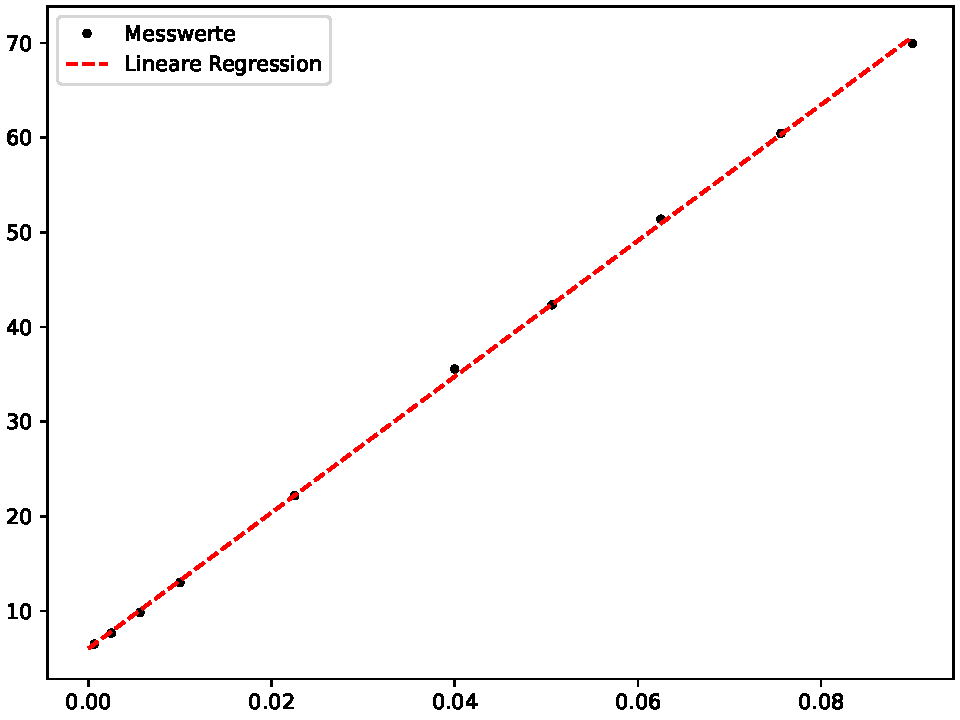
\includegraphics[width=\textwidth]{plot.pdf}
  \caption{Aufgetragen ist die gemittelte, reziproke Periodendauer in Abhängigkeit zur magnetischen Flussdichte.}
  \label{fig:Präzession}
\end{figure}

